% !TEX root = ../main.tex
\section{Messungen und Auswertung}
\label{sec:messungen}

Die Oszillogramme tragen die Zeitstempel des Oszilloskops (13.11.2026 für Aufgabe~6.1.1, 27.11.2026 für die Nachmessung von «3.\ und 5.\ eliminiert» und der Grundfrequenztaktung in Abbildung~\ref{fig:621}, 20.11.2026 für alle weiteren). Die Spuren sind an ihrer Form erkennbar (sinusförmige Netzspannung, pulsförmige Wechselrichterspannung, Netzstrom in Magenta); die Kanalfarben unterscheiden sich zwischen den Messtagen.

% ==========================================================================
\subsection{Aufgabe 6.1.1: Stromform bei Grundfrequenztaktung}
\label{sec:messung611}

Eingestellt wurden $\Th\approx\SI{0}{\degree}$ und $\Udc=\SI{259}{\volt}$. Der Grundschwingungsstrom liess sich nicht auf null bringen; sein Minimum betrug $I_1=\SI{0.827}{\ampere}$, was einer Spannungsdifferenz von rund \SI{18}{\volt} an $X=\SI{22}{\ohm}$ entspricht. Diese Differenz lässt sich mit dem Winkel-Offset aus Abschnitt~\ref{sec:messung612} erklären, sofern er an beiden Messtagen gleich war: Wird $P$ erst bei $\Th\approx\SI{4.7}{\degree}$ null, liegt bei angezeigtem $\Th\approx0$ effektiv ein Winkel von etwa \SI{4.7}{\degree} zwischen den Spannungen. Das ergibt $\Delta U\approx\SI{233}{\volt}\cdot\sin\SI{4.7}{\degree}\approx\SI{19}{\volt}$ und $I_1\approx\SI{0.87}{\ampere}$, was gut zum gemessenen Minimum passt (berechnet). Abbildung~\ref{fig:611} zeigt die Verläufe.

\begin{figure}[htbp]
  \centering
  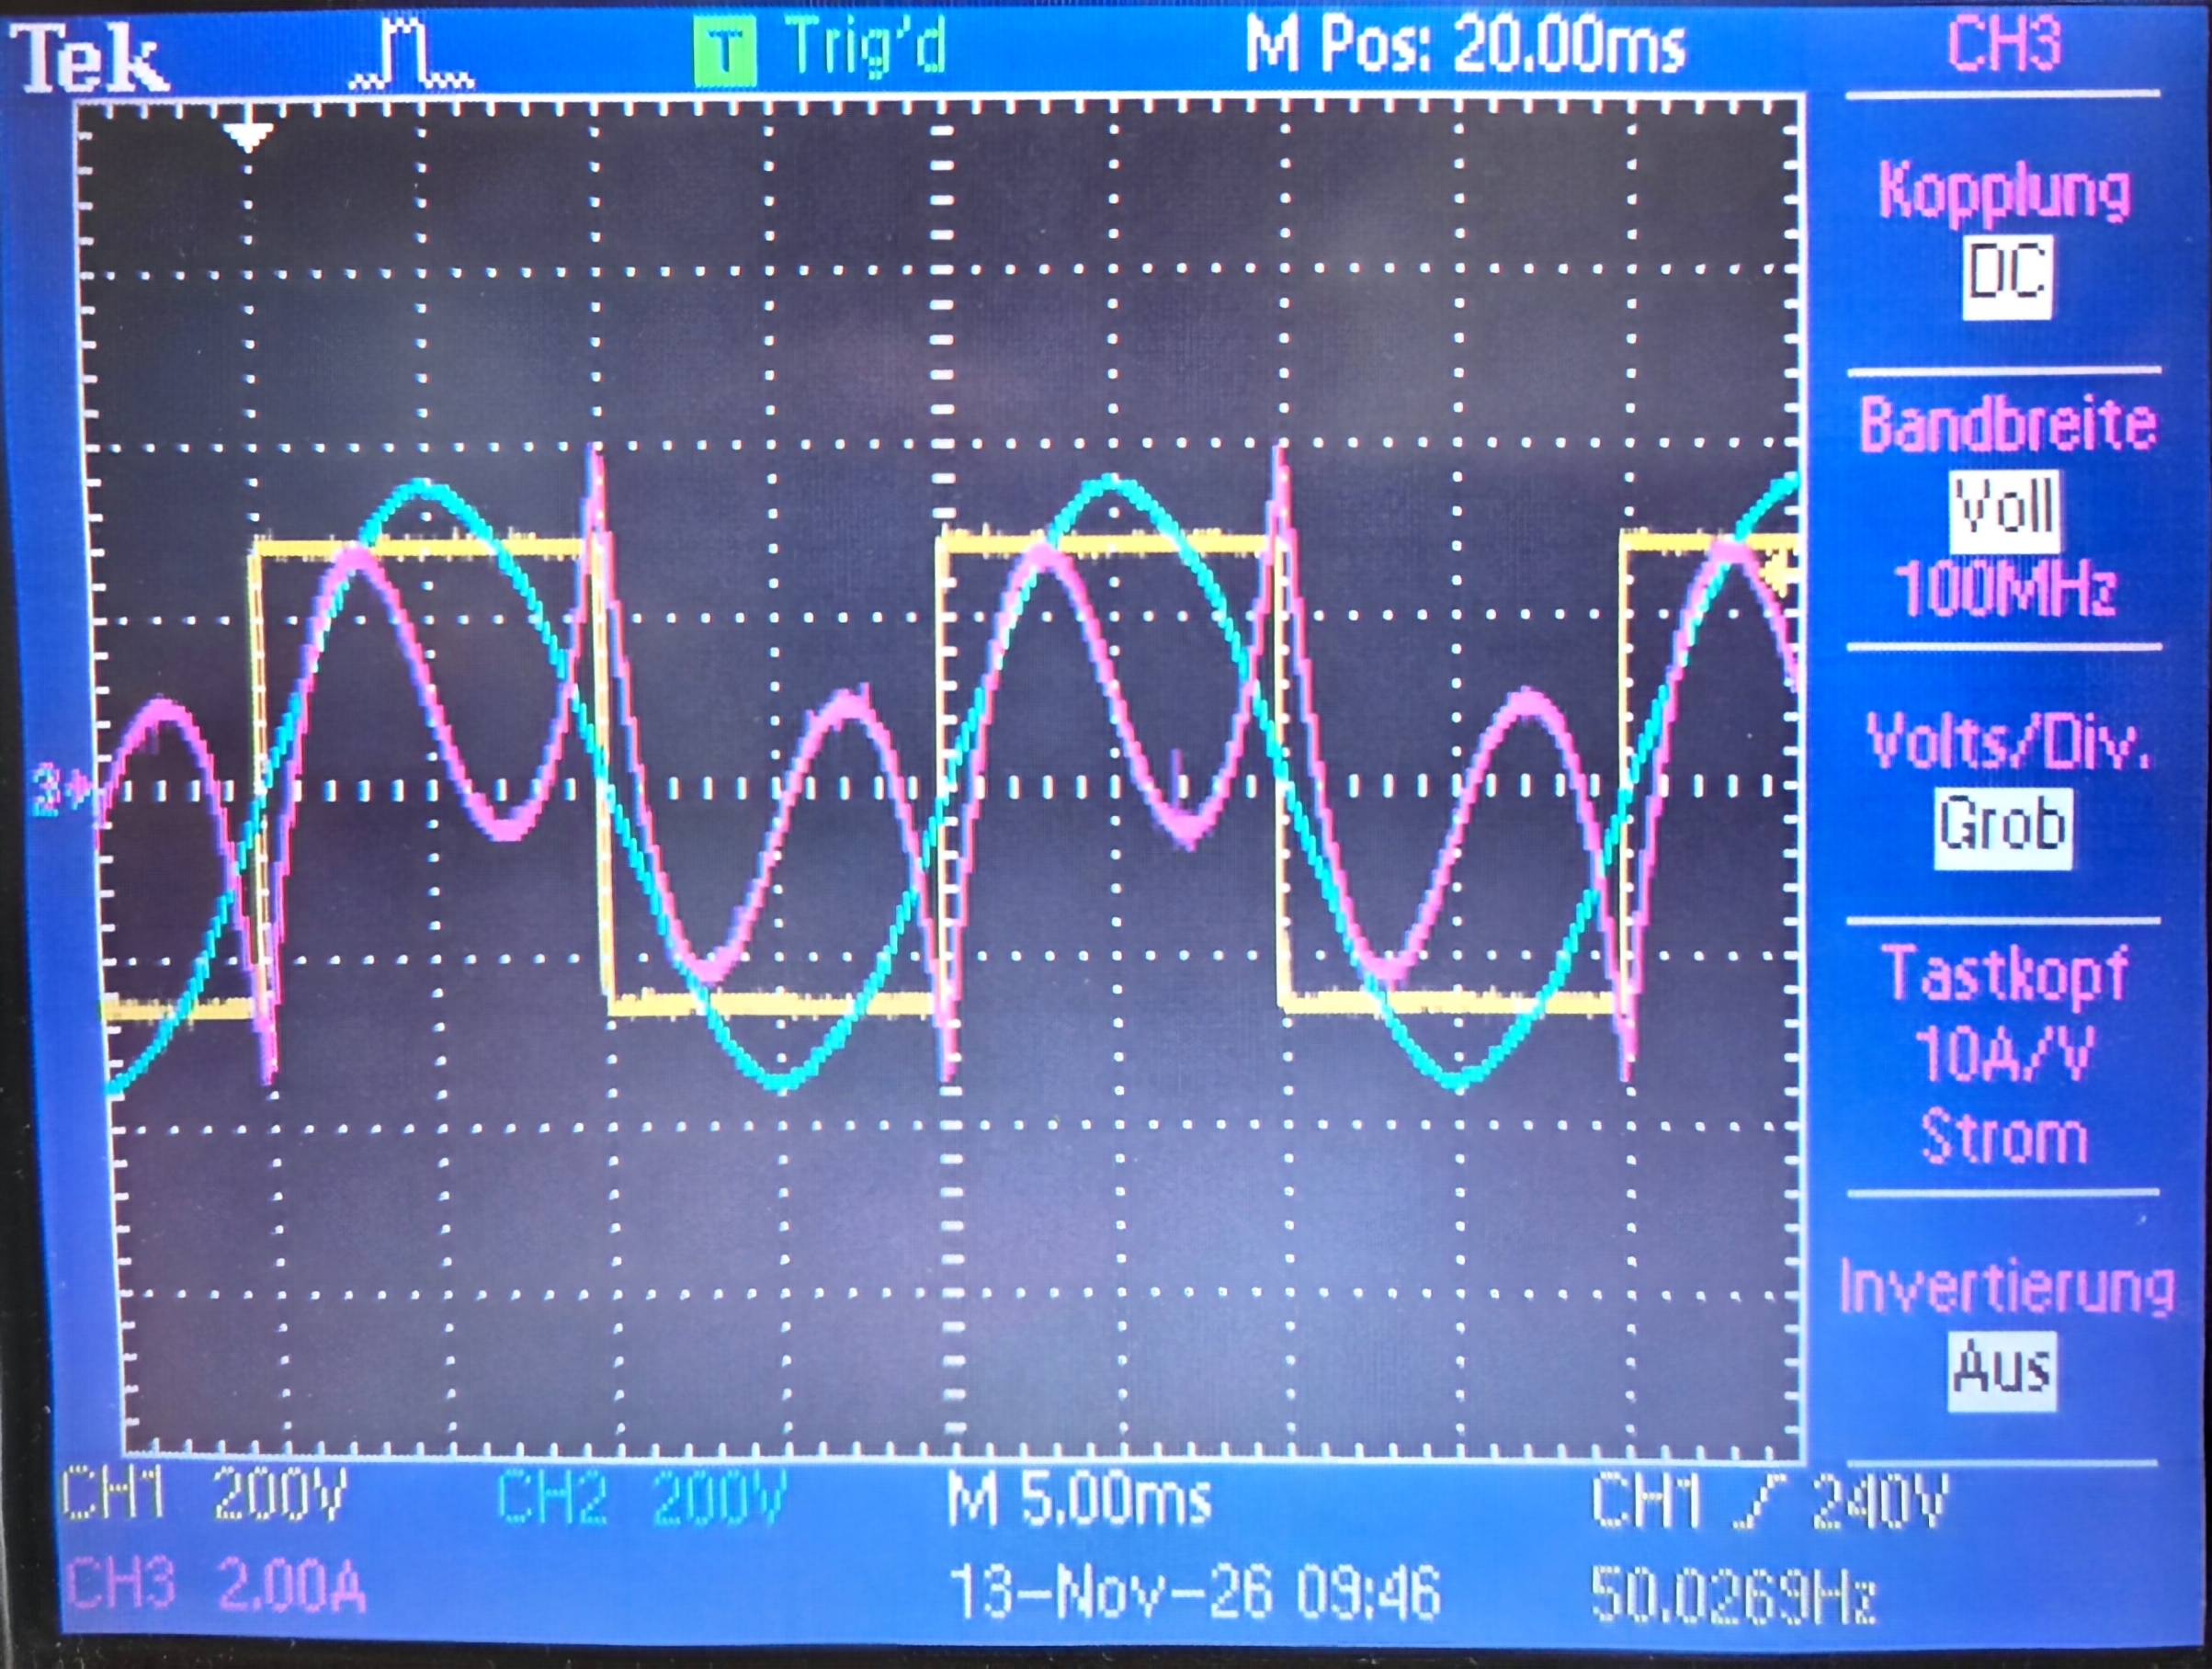
\includegraphics[width=0.62\linewidth]{Scan_20261113_101112.jpg}
  \caption{Aufgabe 6.1.1, Grundfrequenztaktung bei $\Udc=\SI{259}{\volt}$, $\Th\approx\SI{0}{\degree}$ (13.11.2026): rechteckförmige Wechselrichterspannung, sinusförmige Netzspannung und Netzstrom (Magenta). Skalen: \SI{200}{\volt}/div, \SI{2}{\ampere}/div, \SI{5}{\milli\second}/div.}
  \label{fig:611}
\end{figure}

Der Strom hat die erwartete Form aus Abschnitt~\ref{sec:vorbereitung}: Er besteht im Wesentlichen aus Oberschwingungen, und bei den Schaltflanken sind Stromspitzen zu erkennen. Tabelle~\ref{tab:611} vergleicht die am PM\,3000 abgelesenen Harmonischen mit der Theorie nach \eqref{eq:rechteck} und \eqref{eq:In}. Die Spannungsoberschwingungen wurden in Stellung «WR» gemessen, die Stromoberschwingungen in Stellung «Netz».

\begin{table}[htbp]
  \centering
  \caption{Oberschwingungen bei Grundfrequenztaktung, $\Udc=\SI{259}{\volt}$. $U_n$ in \% von $U_1$, $I_n$ in \% von $I_1=\SI{0.827}{\ampere}$. Theoretisch ist $I_1=0$ für $U_{\mathrm{WR1}}=\UN$ und $\Th=0$; der gemessene Restwert lässt sich mit dem Winkel-Offset erklären (siehe Text).}
  \label{tab:611}
  \begin{tabular}{@{}llrrrr@{}}
    \toprule
    & Ordnung $n$ & 1 & 3 & 5 & 7 \\
    \midrule
    $U_n$ & gemessen & \SI{233.3}{\volt} & \SI{33.42}{\percent} & \SI{19.87}{\percent} & \SI{14.32}{\percent} \\
    $U_n$ & Theorie ($0.9\,\Udc/n$) & \SI{233.1}{\volt} & \SI{33.3}{\percent} & \SI{20.0}{\percent} & \SI{14.3}{\percent} \\
    \midrule
    $I_n$ & gemessen & \SI{0.827}{\ampere} & \SI{145}{\percent} & \SI{50.5}{\percent} & \SI{28.4}{\percent} \\
    $I_n$ & Theorie & $\approx0$ (ideal) & \SI{142}{\percent} & \SI{51}{\percent} & \SI{26}{\percent} \\
    \bottomrule
  \end{tabular}
\end{table}

Spannung und Strom stimmen sehr gut mit der Theorie überein. Die Spannungsoberschwingungen fallen mit $1/n$, die Stromoberschwingungen mit $1/n^2$ ab. Die Abweichung der 7.\ Stromharmonischen (28.4 gegenüber 26\,\%) liegt vermutlich im Bereich der Ablesegenauigkeit.

% ==========================================================================
\subsection{Aufgabe 6.1.2: Einstellen von Wirk- und Blindleistung}
\label{sec:messung612}

Die Vorzeichenkonvention von $P$ und $\Th$ steht in Abschnitt~\ref{sec:vorzeichen}.

Abbildung~\ref{fig:zeiger612} zeigt qualitativ, wie sich die Zeiger und damit die Leistungen in den beiden Messreihen verändern. Wird nur $\Th$ verstellt (oben), dreht sich $\underline U_{\mathrm{WR1}}$ bei gleicher Länge um den Ursprung. Der Spannungsabfall $\Delta\underline U$ an der Induktivität steht dann nahezu senkrecht auf $\underline U_{\mathrm N}$, und der um \SI{90}{\degree} nacheilende Strom liegt fast in Phase ($\Th>0$, Bezug aus dem Netz) oder in Gegenphase ($\Th<0$, Rückspeisung) zur Netzspannung. Der grüne Wirkanteil wächst mit $\sin\Th$, der orange Blindanteil bleibt klein. Wird bei $\Th=0$ nur $\Udc$ und damit die Länge von $\underline U_{\mathrm{WR1}}$ verändert (unten), liegt $\Delta\underline U$ parallel zu $\underline U_{\mathrm N}$, und der Strom steht senkrecht dazu: Es entsteht nur ein Blindanteil. Bei $U_{\mathrm{WR1}}<\UN$ eilt der Strom nach, und der Wechselrichter bezieht induktive Blindleistung (untererregt); bei $U_{\mathrm{WR1}}>\UN$ eilt er vor (übererregt). Dieses Verhalten zeigen auch die Messreihen in den Abbildungen~\ref{fig:Ptheta} und \ref{fig:PUdc}.

\begin{figure}[htbp]
  \centering
  \begin{subfigure}[t]{0.32\linewidth}\centering
  \begin{tikzpicture}[>={Stealth[length=2mm]},scale=0.82,every node/.style={font=\scriptsize}]
    \path[use as bounding box] (-2.0,-1.9) rectangle (3.6,1.9);
    \draw[gray!40] (-1.9,0) -- (3.5,0);
    \draw[->,line width=1.4pt,cP] (0,0) -- (-1.423,0);
    \draw[->,line width=1.4pt,cQ] (-1.423,0) -- (-1.423,-0.251);
    \draw[->,thick,cI] (0,0) -- (-1.423,-0.251) node[above] {$\underline I$};
    \draw[->,thick] (0,0) -- (2.600,0) node[above right=-1pt] {$\underline U_{\mathrm N}$};
    \draw[->,thick,cU] (0,0.0) -- (2.443,0.889) node[above right=-1pt] {$\underline U_{\mathrm{WR1}}$};
    \draw[->,thick,dashed,cD] (2.443,0.889) -- (2.600,0);
    \draw[cU] (1.9,0) arc (0:20:1.9);
    \node[cU] at (2.167,0.382) {$\Th$};
    \node[align=center] at (0.8,-1.65) {\textcolor{cP}{$P<0$}, \textcolor{cQ}{$Q$ klein}};
  \end{tikzpicture}
  \caption{$\Th=\SI{-20}{\degree}$, $U_{\mathrm{WR1}}=\UN$}
  \end{subfigure}
  \hfill
  \begin{subfigure}[t]{0.32\linewidth}\centering
  \begin{tikzpicture}[>={Stealth[length=2mm]},scale=0.82,every node/.style={font=\scriptsize}]
    \path[use as bounding box] (-2.0,-1.9) rectangle (3.6,1.9);
    \draw[gray!40] (-1.9,0) -- (3.5,0);
    \node[cI] at (0.9,-0.45) {$\underline I\approx0$};
    \draw[->,thick] (0,0) -- (2.600,0) node[above right=-1pt] {$\underline U_{\mathrm N}$};
    \draw[->,thick,cU] (0,-0.13) -- (2.600,-0.130) node[below=-1pt] {$\underline U_{\mathrm{WR1}}$};
    \node[align=center] at (0.8,-1.65) {\textcolor{cP}{$P=0$}, \textcolor{cQ}{$Q=0$}};
  \end{tikzpicture}
  \caption{$\Th=\SI{0}{\degree}$, $U_{\mathrm{WR1}}=\UN$}
  \end{subfigure}
  \hfill
  \begin{subfigure}[t]{0.32\linewidth}\centering
  \begin{tikzpicture}[>={Stealth[length=2mm]},scale=0.82,every node/.style={font=\scriptsize}]
    \path[use as bounding box] (-2.0,-1.9) rectangle (3.6,1.9);
    \draw[gray!40] (-1.9,0) -- (3.5,0);
    \draw[->,line width=1.4pt,cP] (0,0) -- (1.423,0);
    \draw[->,line width=1.4pt,cQ] (1.423,0) -- (1.423,-0.251);
    \draw[->,thick,cI] (0,0) -- (1.423,-0.251) node[above] {$\underline I$};
    \draw[->,thick] (0,0) -- (2.600,0) node[above right=-1pt] {$\underline U_{\mathrm N}$};
    \draw[->,thick,cU] (0,0.0) -- (2.443,-0.889) node[below right=-1pt] {$\underline U_{\mathrm{WR1}}$};
    \draw[->,thick,dashed,cD] (2.443,-0.889) -- (2.600,0);
    \draw[cU] (1.9,0) arc (0:-20:1.9);
    \node[cU] at (2.167,-0.382) {$\Th$};
    \node[align=center] at (0.8,-1.65) {\textcolor{cP}{$P>0$}, \textcolor{cQ}{$Q$ klein}};
  \end{tikzpicture}
  \caption{$\Th=\SI{+20}{\degree}$, $U_{\mathrm{WR1}}=\UN$}
  \end{subfigure}

  \medskip
  \begin{subfigure}[t]{0.32\linewidth}\centering
  \begin{tikzpicture}[>={Stealth[length=2mm]},scale=0.82,every node/.style={font=\scriptsize}]
    \path[use as bounding box] (-2.0,-1.9) rectangle (3.6,1.9);
    \draw[gray!40] (-1.9,0) -- (3.5,0);
    \draw[->,line width=1.4pt,cQ] (0.000,0) -- (0.000,-0.832);
    \draw[->,thick,cI] (0,0) -- (0.000,-0.832) node[right] {$\underline I$};
    \draw[->,thick] (0,0) -- (2.600,0) node[above right=-1pt] {$\underline U_{\mathrm N}$};
    \draw[->,thick,cU] (0,-0.13) -- (2.080,-0.130) node[below=-1pt] {$\underline U_{\mathrm{WR1}}$};
    \draw[->,thick,dashed,cD] (2.080,-0.130) -- (2.600,-0.130);
    \node[align=center] at (0.8,-1.65) {\textcolor{cP}{$P=0$}, \textcolor{cQ}{$Q>0$ (untererregt)}};
  \end{tikzpicture}
  \caption{$\Th=\SI{0}{\degree}$, $U_{\mathrm{WR1}}<\UN$ ($\Udc$ klein)}
  \end{subfigure}
  \hfill
  \begin{subfigure}[t]{0.32\linewidth}\centering
  \begin{tikzpicture}[>={Stealth[length=2mm]},scale=0.82,every node/.style={font=\scriptsize}]
    \path[use as bounding box] (-2.0,-1.9) rectangle (3.6,1.9);
    \draw[gray!40] (-1.9,0) -- (3.5,0);
    \node[cI] at (0.9,-0.45) {$\underline I\approx0$};
    \draw[->,thick] (0,0) -- (2.600,0) node[above right=-1pt] {$\underline U_{\mathrm N}$};
    \draw[->,thick,cU] (0,-0.13) -- (2.600,-0.130) node[below=-1pt] {$\underline U_{\mathrm{WR1}}$};
    \node[align=center] at (0.8,-1.65) {\textcolor{cP}{$P=0$}, \textcolor{cQ}{$Q=0$}};
  \end{tikzpicture}
  \caption{$\Th=\SI{0}{\degree}$, $U_{\mathrm{WR1}}=\UN$}
  \end{subfigure}
  \hfill
  \begin{subfigure}[t]{0.32\linewidth}\centering
  \begin{tikzpicture}[>={Stealth[length=2mm]},scale=0.82,every node/.style={font=\scriptsize}]
    \path[use as bounding box] (-2.0,-1.9) rectangle (3.6,1.9);
    \draw[gray!40] (-1.9,0) -- (3.5,0);
    \draw[->,line width=1.4pt,cQ] (0.000,0) -- (0.000,0.832);
    \draw[->,thick,cI] (0,0) -- (0.000,0.832) node[right] {$\underline I$};
    \draw[->,thick] (0,0) -- (2.600,0) node[above right=-1pt] {$\underline U_{\mathrm N}$};
    \draw[->,thick,cU] (0,-0.13) -- (3.120,-0.130) node[below=-1pt] {$\underline U_{\mathrm{WR1}}$};
    \draw[->,thick,dashed,cD] (3.120,0.130) -- (2.600,0.130);
    \node[align=center] at (0.8,-1.65) {\textcolor{cP}{$P=0$}, \textcolor{cQ}{$Q<0$ (übererregt)}};
  \end{tikzpicture}
  \caption{$\Th=\SI{0}{\degree}$, $U_{\mathrm{WR1}}>\UN$ ($\Udc$ gross)}
  \end{subfigure}

  \medskip
  \begin{tikzpicture}[>={Stealth[length=2mm]},every node/.style={font=\scriptsize}]
    \draw[->,thick] (0,0) -- (0.6,0) node[right] {$\underline U_{\mathrm N}$};
    \draw[->,thick,cU] (1.6,0) -- (2.2,0) node[right] {$\underline U_{\mathrm{WR1}}$};
    \draw[->,thick,dashed,cD] (3.5,0) -- (4.1,0) node[right] {$\Delta\underline U=\mathrm jX\underline I$};
    \draw[->,thick,cI] (6.3,0) -- (6.9,0) node[right] {$\underline I$};
    \draw[->,line width=1.4pt,cP] (7.6,0) -- (8.2,0) node[right] {Wirkanteil ($P$)};
    \draw[->,line width=1.4pt,cQ] (10.9,0) -- (11.5,0) node[right] {Blindanteil ($Q$)};
  \end{tikzpicture}
  \caption{Zeigerdiagramme zur Einstellung der Leistungen (qualitativ, $\underline I$ vergrössert dargestellt). Oben: Variation des Winkels $\Th$ bei gleicher Amplitude. $\underline U_{\mathrm{WR1}}$ dreht sich um $\underline U_{\mathrm N}$, $\Delta\underline U$ steht fast senkrecht auf $\underline U_{\mathrm N}$, und der Strom liegt fast in Phase oder Gegenphase zu $\underline U_{\mathrm N}$: Es fliesst hauptsächlich Wirkleistung, deren Vorzeichen mit $\Th$ wechselt. Unten: Variation der Amplitude über $\Udc$ bei $\Th=0$. $\Delta\underline U$ liegt parallel zu $\underline U_{\mathrm N}$, der Strom steht senkrecht dazu: Es fliesst nur Blindleistung, deren Vorzeichen davon abhängt, ob $U_{\mathrm{WR1}}$ kleiner oder grösser als $\UN$ ist.}
  \label{fig:zeiger612}
\end{figure}


\paragraph{\texorpdfstring{Variation von $\Th$ bei $\Udc=\SI{258.7}{\volt}$}{Variation von Theta bei Udc = 258.7 V}.}

\begin{table}[htbp]
  \centering
  \caption{Gemessene Leistungen in Abhängigkeit von $\Th$, $\Udc=\SI{258.7}{\volt}$.}
  \label{tab:theta}
  \begin{tabular}{@{}rrr@{}}
    \toprule
    $\Th$ in \si{\degree} & $P$ in W & $Q$ in var \\
    \midrule
    $-20$ & $-1057.5$ & 480.7 \\
    $-10$ & $-660$ & 384.9 \\
    0 & $-210$ & 329.5 \\
    10 & 240 & 321.9 \\
    20 & 678 & 360 \\
    \bottomrule
  \end{tabular}
\end{table}

\begin{figure}[htbp]
  \centering
  \begin{tikzpicture}
    \begin{axis}[rep,xlabel={$\Th$ in \si{\degree}},ylabel={$P$ in W, $Q$ in var},
        legend pos=north west,xmin=-25,xmax=25]
      \addplot[thick,mark=*] table[x=theta_deg,y=P_W,col sep=comma]{data/theta_reihe.csv};
      \addlegendentry{$P$}
      \addplot[thick,dashed,mark=square*] table[x=theta_deg,y=Q_var,col sep=comma]{data/theta_reihe.csv};
      \addlegendentry{$Q$}
    \end{axis}
  \end{tikzpicture}
  \caption{$P(\Th)$ und $Q(\Th)$ bei $\Udc=\SI{258.7}{\volt}$ (Messwerte aus Tabelle~\ref{tab:theta}).}
  \label{fig:Ptheta}
\end{figure}

$P$ verläuft ungefähr proportional zu $\sin\Th$ (Abbildung~\ref{fig:Ptheta}). Nach \eqref{eq:PQ} wäre für $\Th=\SI{20}{\degree}$ mit $\UN=\SI{230}{\volt}$, $U_{\mathrm{WR1}}=\SI{233}{\volt}$ und $X=\SI{22}{\ohm}$ eine Leistung von etwa \SI{833}{\watt} zu erwarten. Gemessen ist die halbe Differenz zwischen $+\SI{20}{\degree}$ und $-\SI{20}{\degree}$ gleich \SI{868}{\watt} (berechnet aus Tabelle~\ref{tab:theta}), also rund \SI{4}{\percent} mehr. Die Kurve ist allerdings nicht um $\Th=0$ zentriert: $P=0$ liegt nach linearer Interpolation zwischen $\SI{0}{\degree}$ und $\SI{10}{\degree}$ bei $\Th\approx\SI{4.7}{\degree}$. Dazu passt die Notiz, dass der Strom bei $\SI{4.1}{\degree}$ und \SI{263}{\volt} am kleinsten war. Für diesen Winkel-Offset gibt es keine gesicherte Erklärung. Mögliche Ursachen sind die Synchronisation, Verluste in Wechselrichter, Drossel und Transformator oder Messtoleranzen (Vermutungen, nicht überprüft).

$Q$ ändert sich in $\Th$ nur wenig und hat sein Minimum zwischen $\SI{0}{\degree}$ und $\SI{10}{\degree}$. Es erreicht nie null, weil $Q$ am PM\,3000 die Verzerrungsblindleistung enthält.

\paragraph{\texorpdfstring{Variation von $\Udc$ bei $\Th=\SI{0}{\degree}$}{Variation von Udc bei Theta = 0 Grad}.}

\begin{table}[htbp]
  \centering
  \caption{Gemessene Leistungen in Abhängigkeit von $\Udc$, $\Th=\SI{0}{\degree}$.}
  \label{tab:udc}
  \begin{tabular}{@{}rrr@{}}
    \toprule
    $\Udc$ in V & $P$ in W & $Q$ in var \\
    \midrule
    150 & $-62.63$ & 1134 \\
    175 & $-87.68$ & 911 \\
    200 & $-116$ & 670 \\
    225 & $-150$ & 476 \\
    250 & $-192.6$ & 340 \\
    275 & $-234$ & 350 \\
    300 & $-266$ & 530 \\
    325 & $-298$ & 720 \\
    350 & $-320$ & nicht notiert \\
    \bottomrule
  \end{tabular}
\end{table}

Der Wert von $Q$ bei \SI{350}{\volt} wurde nicht notiert.

\begin{figure}[htbp]
  \centering
  \begin{tikzpicture}
    \begin{axis}[rep,xlabel={$\Udc$ in V},ylabel={$P$ in W, $Q$ in var},
        legend pos=north east,xmin=125,xmax=375]
      \addplot[thick,mark=*] table[x=udc_V,y=P_W,col sep=comma]{data/udc_reihe.csv};
      \addlegendentry{$P$}
      \addplot[thick,dashed,mark=square*] table[x=udc_V,y=Q_var,col sep=comma]{data/udc_reihe.csv};
      \addlegendentry{$Q$}
    \end{axis}
  \end{tikzpicture}
  \caption{$P(\Udc)$ und $Q(\Udc)$ bei $\Th=\SI{0}{\degree}$ (Messwerte aus Tabelle~\ref{tab:udc}).}
  \label{fig:PUdc}
\end{figure}

$Q$ hat ein Minimum bei $\Udc\approx\SI{250}{\volt}$ bis \SI{275}{\volt}. Dort ist $U_{\mathrm{WR1}}\approx\UN$; nach \eqref{eq:rechteck} gilt dies für $\Udc=\SI{230}{\volt}/0.9\approx\SI{256}{\volt}$. Unterhalb dieses Bereichs ist der Wechselrichter untererregt, oberhalb übererregt. Weil das gemessene $Q$ ein Betrag mit Verzerrungsanteil ist, entsteht ein V-förmiges Minimum und kein Nulldurchgang; erst $Q_1$ würde das Vorzeichen wechseln. $P$ ändert sich mit $\Udc$ nur leicht. Da $\Th=0$ nicht der Nullpunkt von $P$ ist (Offset von $\approx\SI{4.7}{\degree}$, siehe oben), nimmt $|P|$ mit $\Udc$ etwa linear zu. Proportional ist der Zusammenhang allerdings nicht: $|P|/\Udc$ steigt von \SI{0.42}{\watt\per\volt} bei \SI{150}{\volt} auf \SI{0.91}{\watt\per\volt} bei \SI{350}{\volt}, und eine Ausgleichsgerade durch die Messpunkte erreicht $P=0$ erst bei rund \SI{110}{\volt} (berechnet). Die Ursache wurde nicht untersucht; denkbar sind Verluste oder ein vom Betriebspunkt abhängiger Winkel-Offset (Vermutung).

\paragraph{Grundschwingungsgrössen und Harmonische.} Die Grössen $P_1$, $Q_1$ und $I_3$ wurden in beiden Messreihen nicht aufgenommen. Wegen $P\approx P_1$ (Netzspannung nahezu sinusförmig) liegen die $P_1$-Kurven praktisch auf den $P$-Kurven. $Q_1$ lässt sich qualitativ über das Minimum der $Q$-Kurve diskutieren: Dort wechselt $Q_1$ das Vorzeichen. Dass das Minimum von $Q$ nicht bei null, sondern bei rund \SI{320}{\VAr} bis \SI{340}{\VAr} liegt, lässt sich mit der Verzerrungsblindleistung $D=\UN\,I_{\mathrm h}$ erklären, wobei $I_{\mathrm h}=\sqrt{\sum_{n\ge3}I_n^2}$ der Oberschwingungsstrom ist. Mit $I_n=0.9\,\Udc/(n^2X)$ nach \eqref{eq:rechteck} und \eqref{eq:In} und $\sum_{n=3,5,\dots}n^{-4}=\pi^4/96-1\approx0.0147$ ergibt sich für $\Udc=\SI{258.7}{\volt}$ ein Oberschwingungsstrom von $I_{\mathrm h}\approx\SI{1.28}{\ampere}$ und damit $D\approx\SI{295}{\VAr}$ (berechnet, nicht gemessen). Im Minimum ist $Q_1\approx0$ und deshalb $Q\approx D$; der berechnete Wert liegt rund \SI{10}{\percent} unter dem gemessenen Minimum, den Rest erklären vermutlich $Q_1\neq0$ und Oberschwingungen der Netzspannung.

Nach \eqref{eq:rechteck} und \eqref{eq:In} sind die Oberschwingungsamplituden von $\uWR$ proportional zu $\Udc$ und unabhängig von $\Th$ (der Winkel verschiebt nur die Phase). Die Stromoberschwingungen $I_n=U_{\mathrm{WR},n}/(nX)$ sollten deshalb mit $\Udc$ zunehmen und von $\Th$ nicht abhängen; gemessen wurden die Harmonischen in dieser Aufgabe nicht.

% ==========================================================================
\subsection{Aufgabe 6.2.1: Weitere Pulsmuster}
\label{sec:messung621}

Verglichen wurden die Muster «Trägerverfahren fein», «Trägerverfahren grob» und «3.\ und 5.\ eliminiert» (sowie die Grundfrequenztaktung als Referenz) bei einem festen Lastpunkt von $P\approx\SI{1.15}{\kilo\watt}$ und $Q_1\approx0$. Die Anleitung nennt $P=\SI{1.5}{\kilo\watt}$ als Beispiel; dieser Wert wurde nicht angefahren: Das Einpendeln von $P$ und $Q_1\approx0$ durch iteratives Nachstellen von $\Th$ und $\Udc$ war aufwendig, und bei rund \SI{1.1}{\kilo\watt} liess sich $Q_1\approx0$ bei allen Mustern rasch einstellen. Für den Vergleich der Muster zählt nur, dass der Lastpunkt für alle gleich ist, nicht seine Höhe; als gemeinsamer Lastpunkt wurde deshalb $P\approx\SI{1.15}{\kilo\watt}$ verwendet. Eingestellt wurden die Werte in Tabelle~\ref{tab:621_einst}.

\begin{table}[htbp]
  \centering
  \caption{Einstellungen am Lastpunkt $P\approx\SI{1.15}{\kilo\watt}$, $Q_1\approx0$. Die Werte für «3.\ und 5.\ eliminiert» und die Grundfrequenztaktung stammen aus der Nachmessung vom 27.11.2026.}
  \label{tab:621_einst}
  \begin{tabular}{@{}lrr@{}}
    \toprule
    Pulsmuster & $\Udc$ in V & $\Th$ in \si{\degree} \\
    \midrule
    Grundfrequenztaktung & 284 & 28.0 \\
    3.\ und 5.\ eliminiert & 342 & 29.8 \\
    Trägerverfahren fein & 358 & 29.8 \\
    Trägerverfahren grob & 363 & 29.8 \\
    \bottomrule
  \end{tabular}
\end{table}

Alle Muster brauchen dieselbe Grundschwingung $U_{\mathrm{WR1}}$ (gleicher Lastpunkt, gleicher Winkel). Mit dem Winkel-Offset aus Abschnitt~\ref{sec:messung612} ist der wirksame Winkel $\Th_{\mathrm{eff}}\approx\SI{29.8}{\degree}-\SI{4.7}{\degree}=\SI{25.1}{\degree}$. Für $Q_1=0$ muss $U_{\mathrm{WR1}}\cos\Th_{\mathrm{eff}}=\UN$ gelten, also $U_{\mathrm{WR1}}\approx\SI{254}{\volt}$; nach \eqref{eq:PQ} folgt daraus $P\approx\SI{1.13}{\kilo\watt}$, was dem eingestellten Lastpunkt entspricht (berechnet). Damit ist $U_{\mathrm{WR1}}/\Udc$ bei «3.\ und 5.\ eliminiert» $254/342\approx0.74$, beim Trägerverfahren «fein» $254/358\approx0.71$ und bei «grob» $254/363\approx0.70$, gegenüber 0.9 bei der Rechteckspannung. Die Kerben des Musters «3.\ und 5.\ eliminiert» verkleinern die Grundschwingung also auf rund \SI{83}{\percent} des Rechteckwerts, das Trägerverfahren auf knapp \SI{80}{\percent}. Je mehr ein Muster die Rechteckspannung zerteilt, desto schlechter nutzt es die Zwischenkreisspannung aus und desto höher muss $\Udc$ für denselben Lastpunkt sein.

Die Grundfrequenztaktung passt zu dieser Abschätzung: Mit $\Udc=\SI{284}{\volt}$ ist $U_{\mathrm{WR1}}=0.9\cdot\SI{284}{\volt}\approx\SI{256}{\volt}$, also nahezu der oben berechnete Wert. Mit dem wirksamen Winkel $\SI{28.0}{\degree}-\SI{4.7}{\degree}=\SI{23.3}{\degree}$ folgen nach \eqref{eq:PQ} $P\approx\SI{1.06}{\kilo\watt}$ und $Q_1\approx\SI{-50}{\VAr}$ (berechnet), also nahezu derselbe Lastpunkt.

Die Oszillogramme von «3.\ und 5.\ eliminiert» und der Grundfrequenztaktung wurden am 20.11.2026 nicht aufgenommen und deshalb in einer Nachmessung am 27.11.2026 beim gleichen Lastpunkt nachgeholt. Dabei wurden auch die Einstellungen in Tabelle~\ref{tab:621_einst} notiert. Die Oberschwingungsanteile in Tabelle~\ref{tab:621_harm} stammen vom 20.11.2026.

Die gemessenen Oberschwingungen stehen in Tabelle~\ref{tab:621_harm}. Die Spannungsoberschwingungen wurden in Stellung «WR», die Stromoberschwingungen in Stellung «Netz» abgelesen.

\begin{table}[htbp]
  \centering
  \caption{Oberschwingungen der Pulsmuster am Lastpunkt (Angaben in \%, grobe Richtwerte wegen stark schwankender Anzeige, bezogen auf die jeweilige Grundschwingung).}
  \label{tab:621_harm}
  \begin{tabular}{@{}lrrrr@{}}
    \toprule
    Pulsmuster & $U_3$ & $U_5$ & $I_3$ & $I_5$ \\
    \midrule
    Trägerverfahren fein & 20 & 10 & 20 & 30 \\
    Trägerverfahren grob & 30 & 12 & 22 & 10 \\
    3.\ und 5.\ eliminiert & 0.5 & 30 & 9 & 7 \\
    \bottomrule
  \end{tabular}
\end{table}

Die Prozentwerte des PM\,3000 beziehen sich auf die jeweilige Grundschwingung. Das zeigt die Messung in Tabelle~\ref{tab:611}: Dort ist $I_3=\SI{145}{\percent}$, was nur bei Bezug auf $I_1$ möglich ist, und der Wert stimmt mit der Theorie (\SI{142}{\percent}) überein.

Die Oszillogramme der drei Muster und, als Referenz, der Grundfrequenztaktung zeigt Abbildung~\ref{fig:621}.

\begin{figure}[htbp]
  \centering
  \begin{subfigure}[t]{0.48\linewidth}
    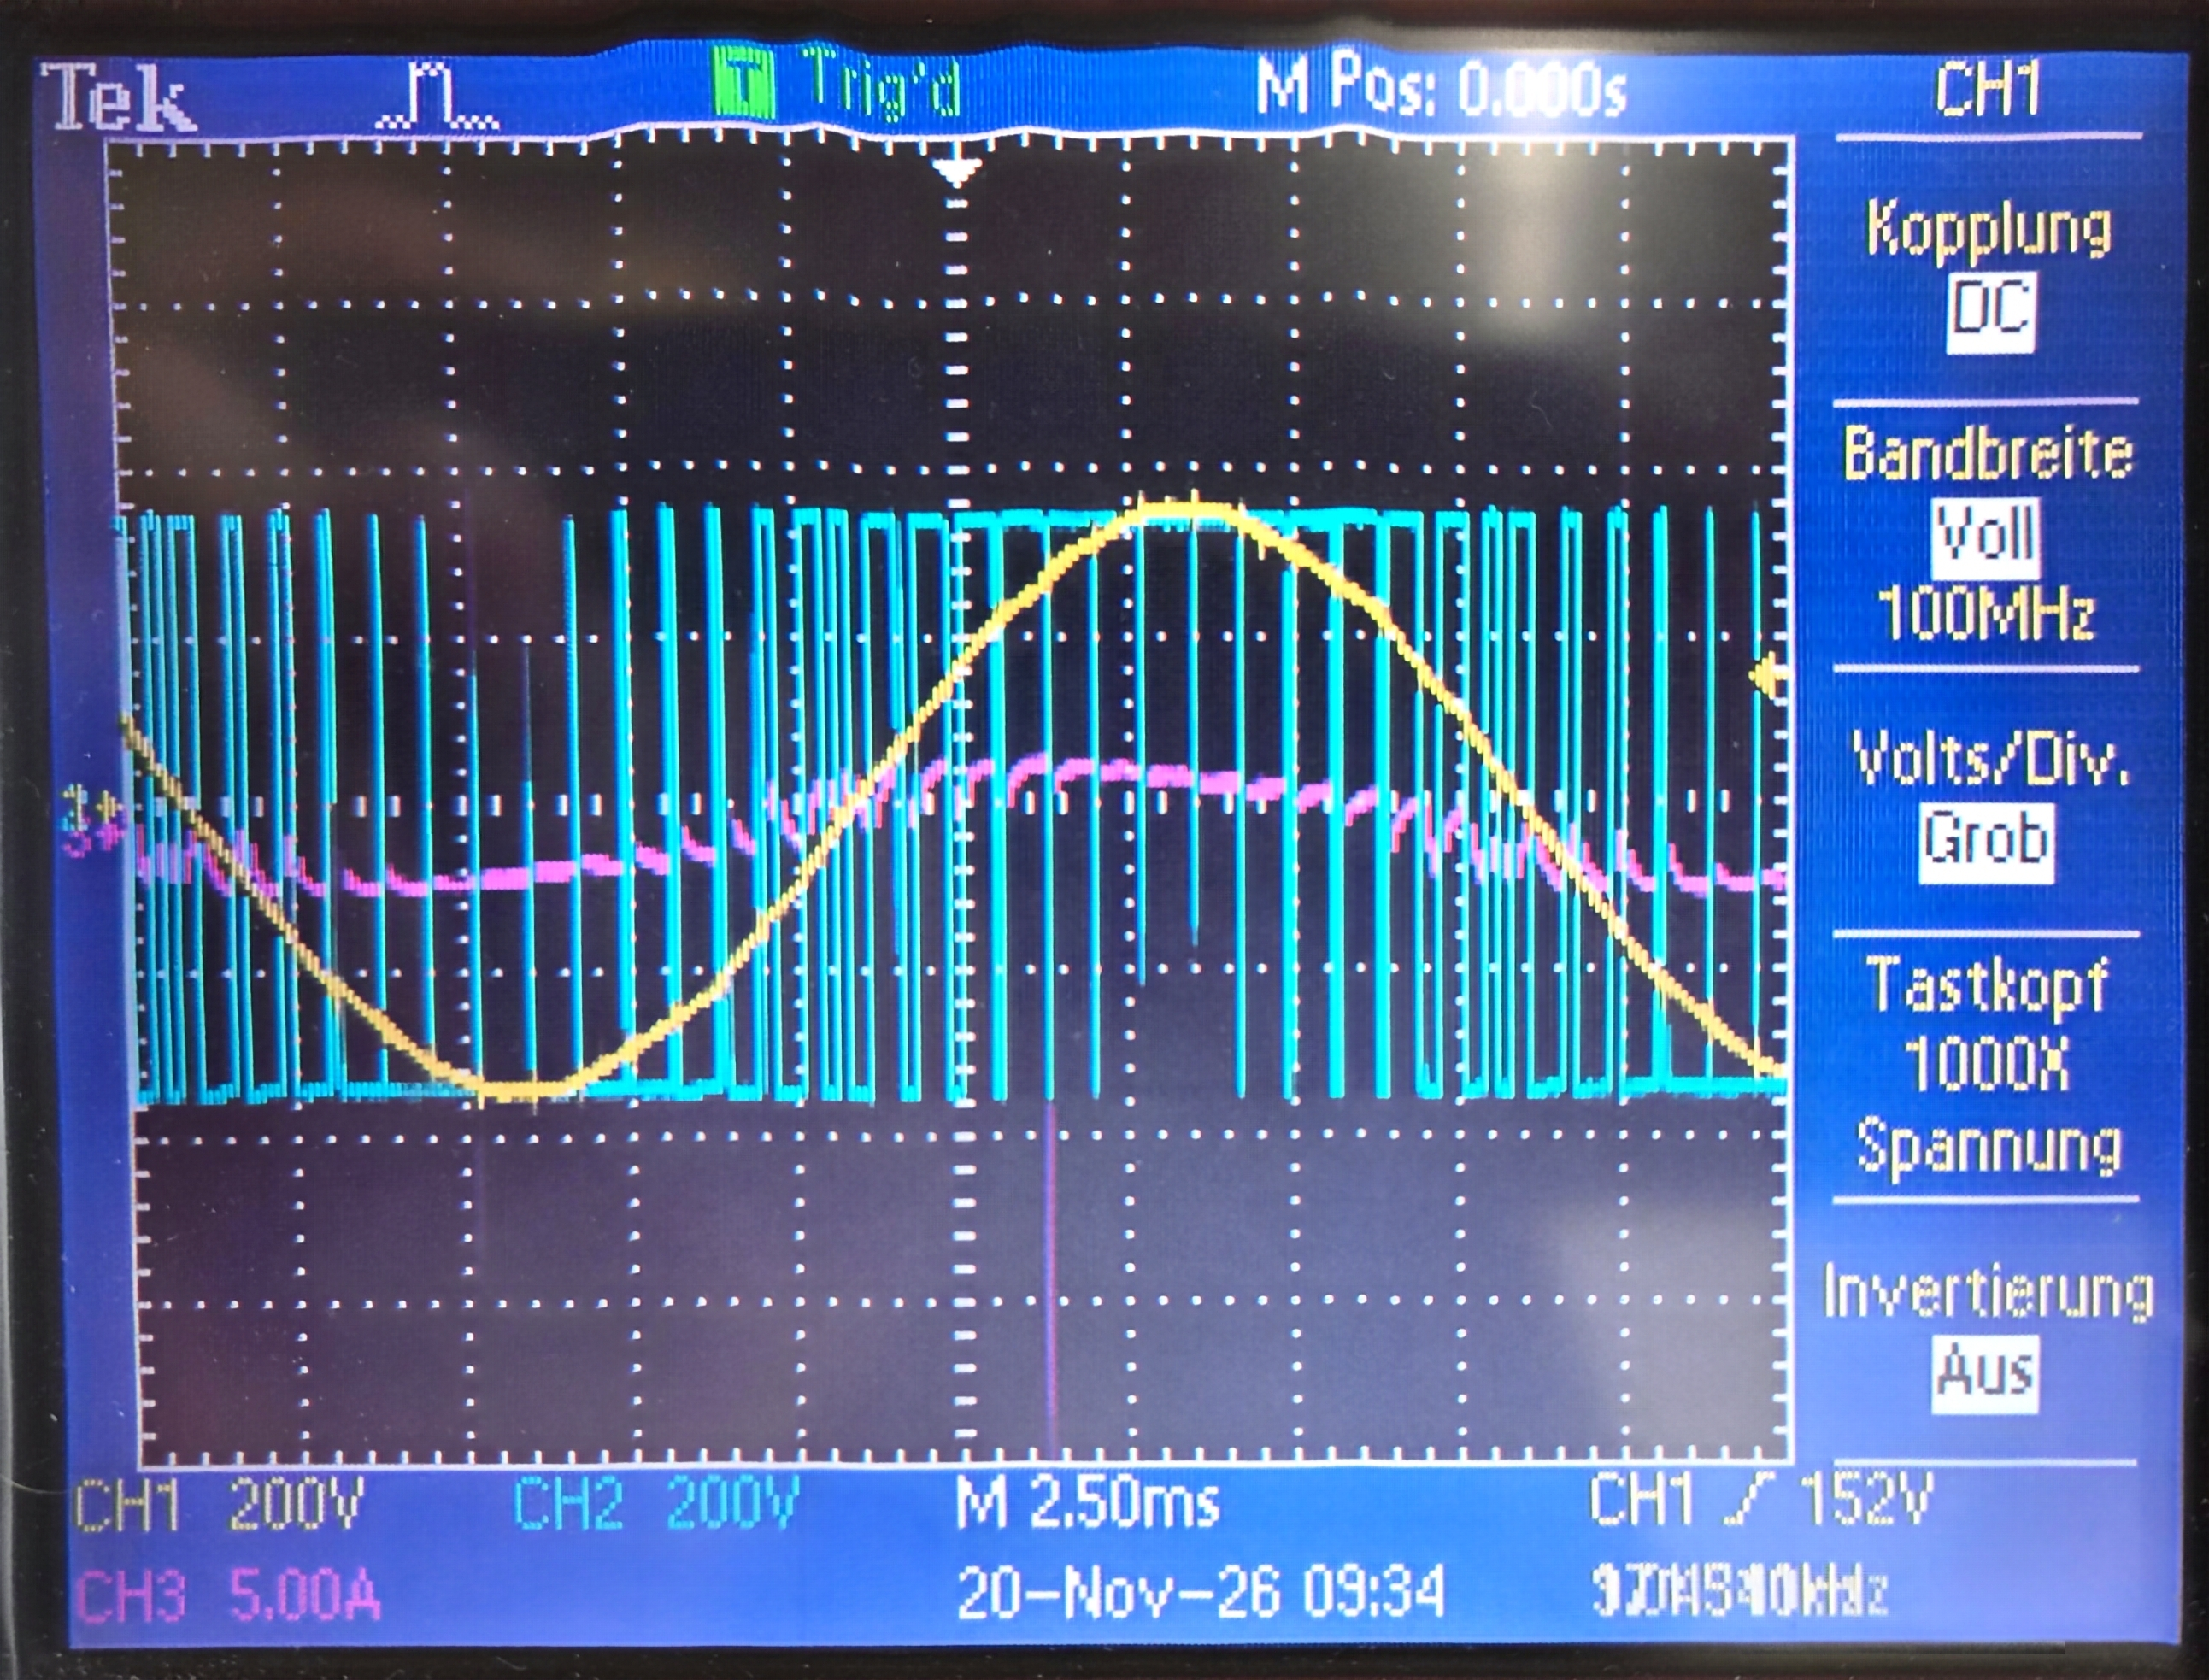
\includegraphics[width=\linewidth]{Scan_20261120_095904.jpg}
    \caption{Trägerverfahren fein, $\Udc=\SI{358}{\volt}$}
    \label{fig:621_fein}
  \end{subfigure}\hfill
  \begin{subfigure}[t]{0.48\linewidth}
    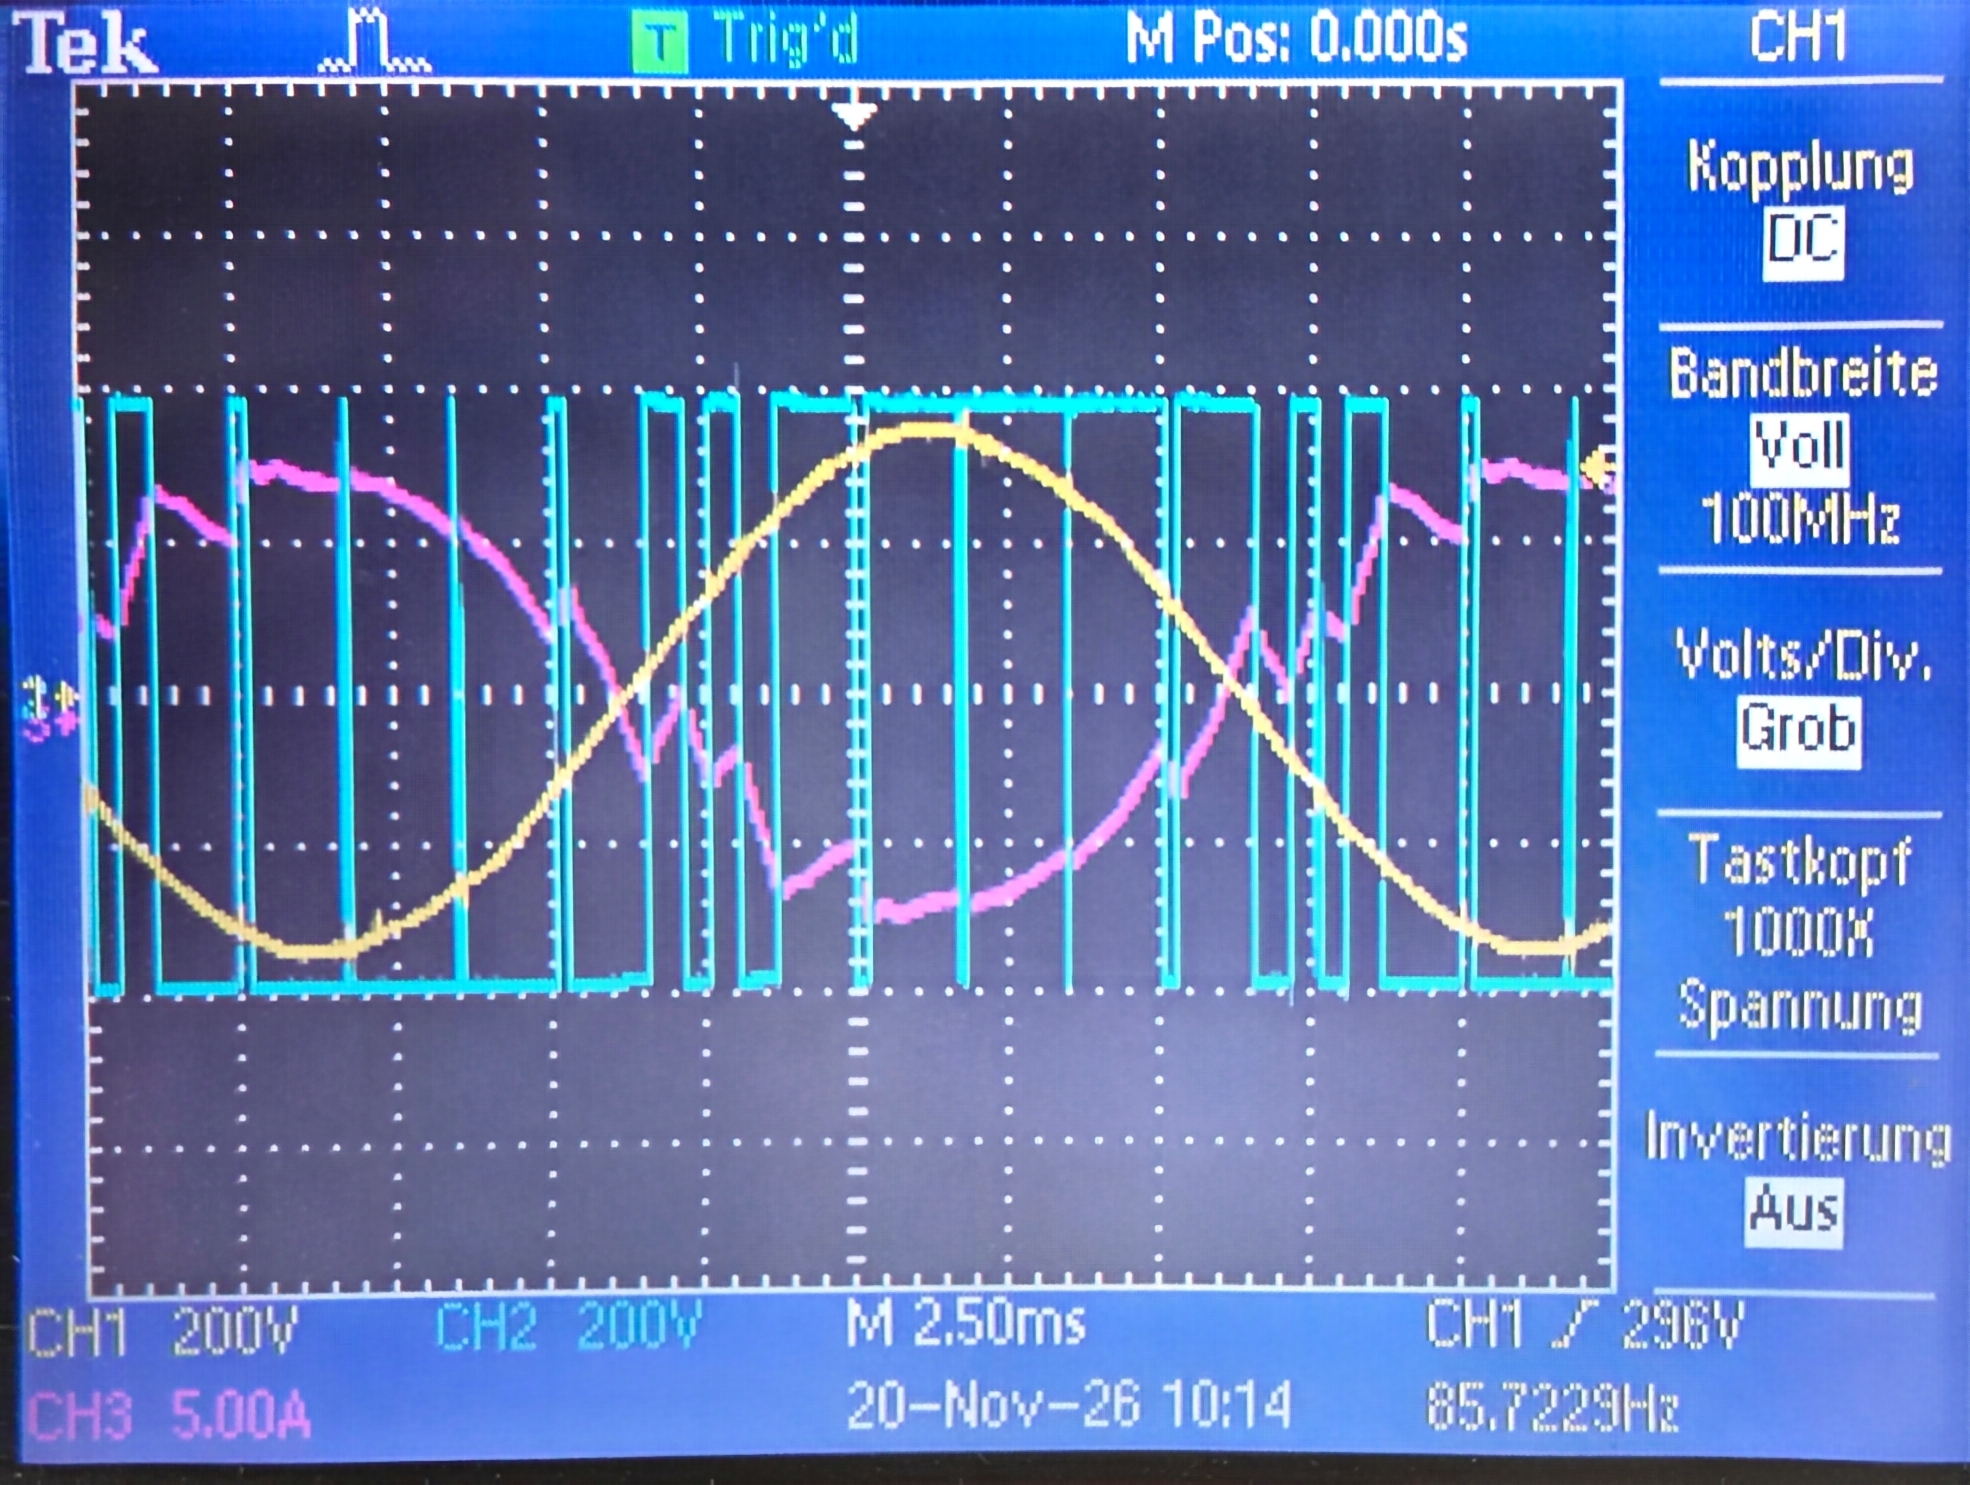
\includegraphics[width=\linewidth]{Scan_20261120_103938.jpg}
    \caption{Trägerverfahren grob, $\Udc=\SI{363}{\volt}$}
    \label{fig:621_grob}
  \end{subfigure}

  \medskip
  \begin{subfigure}[t]{0.48\linewidth}
    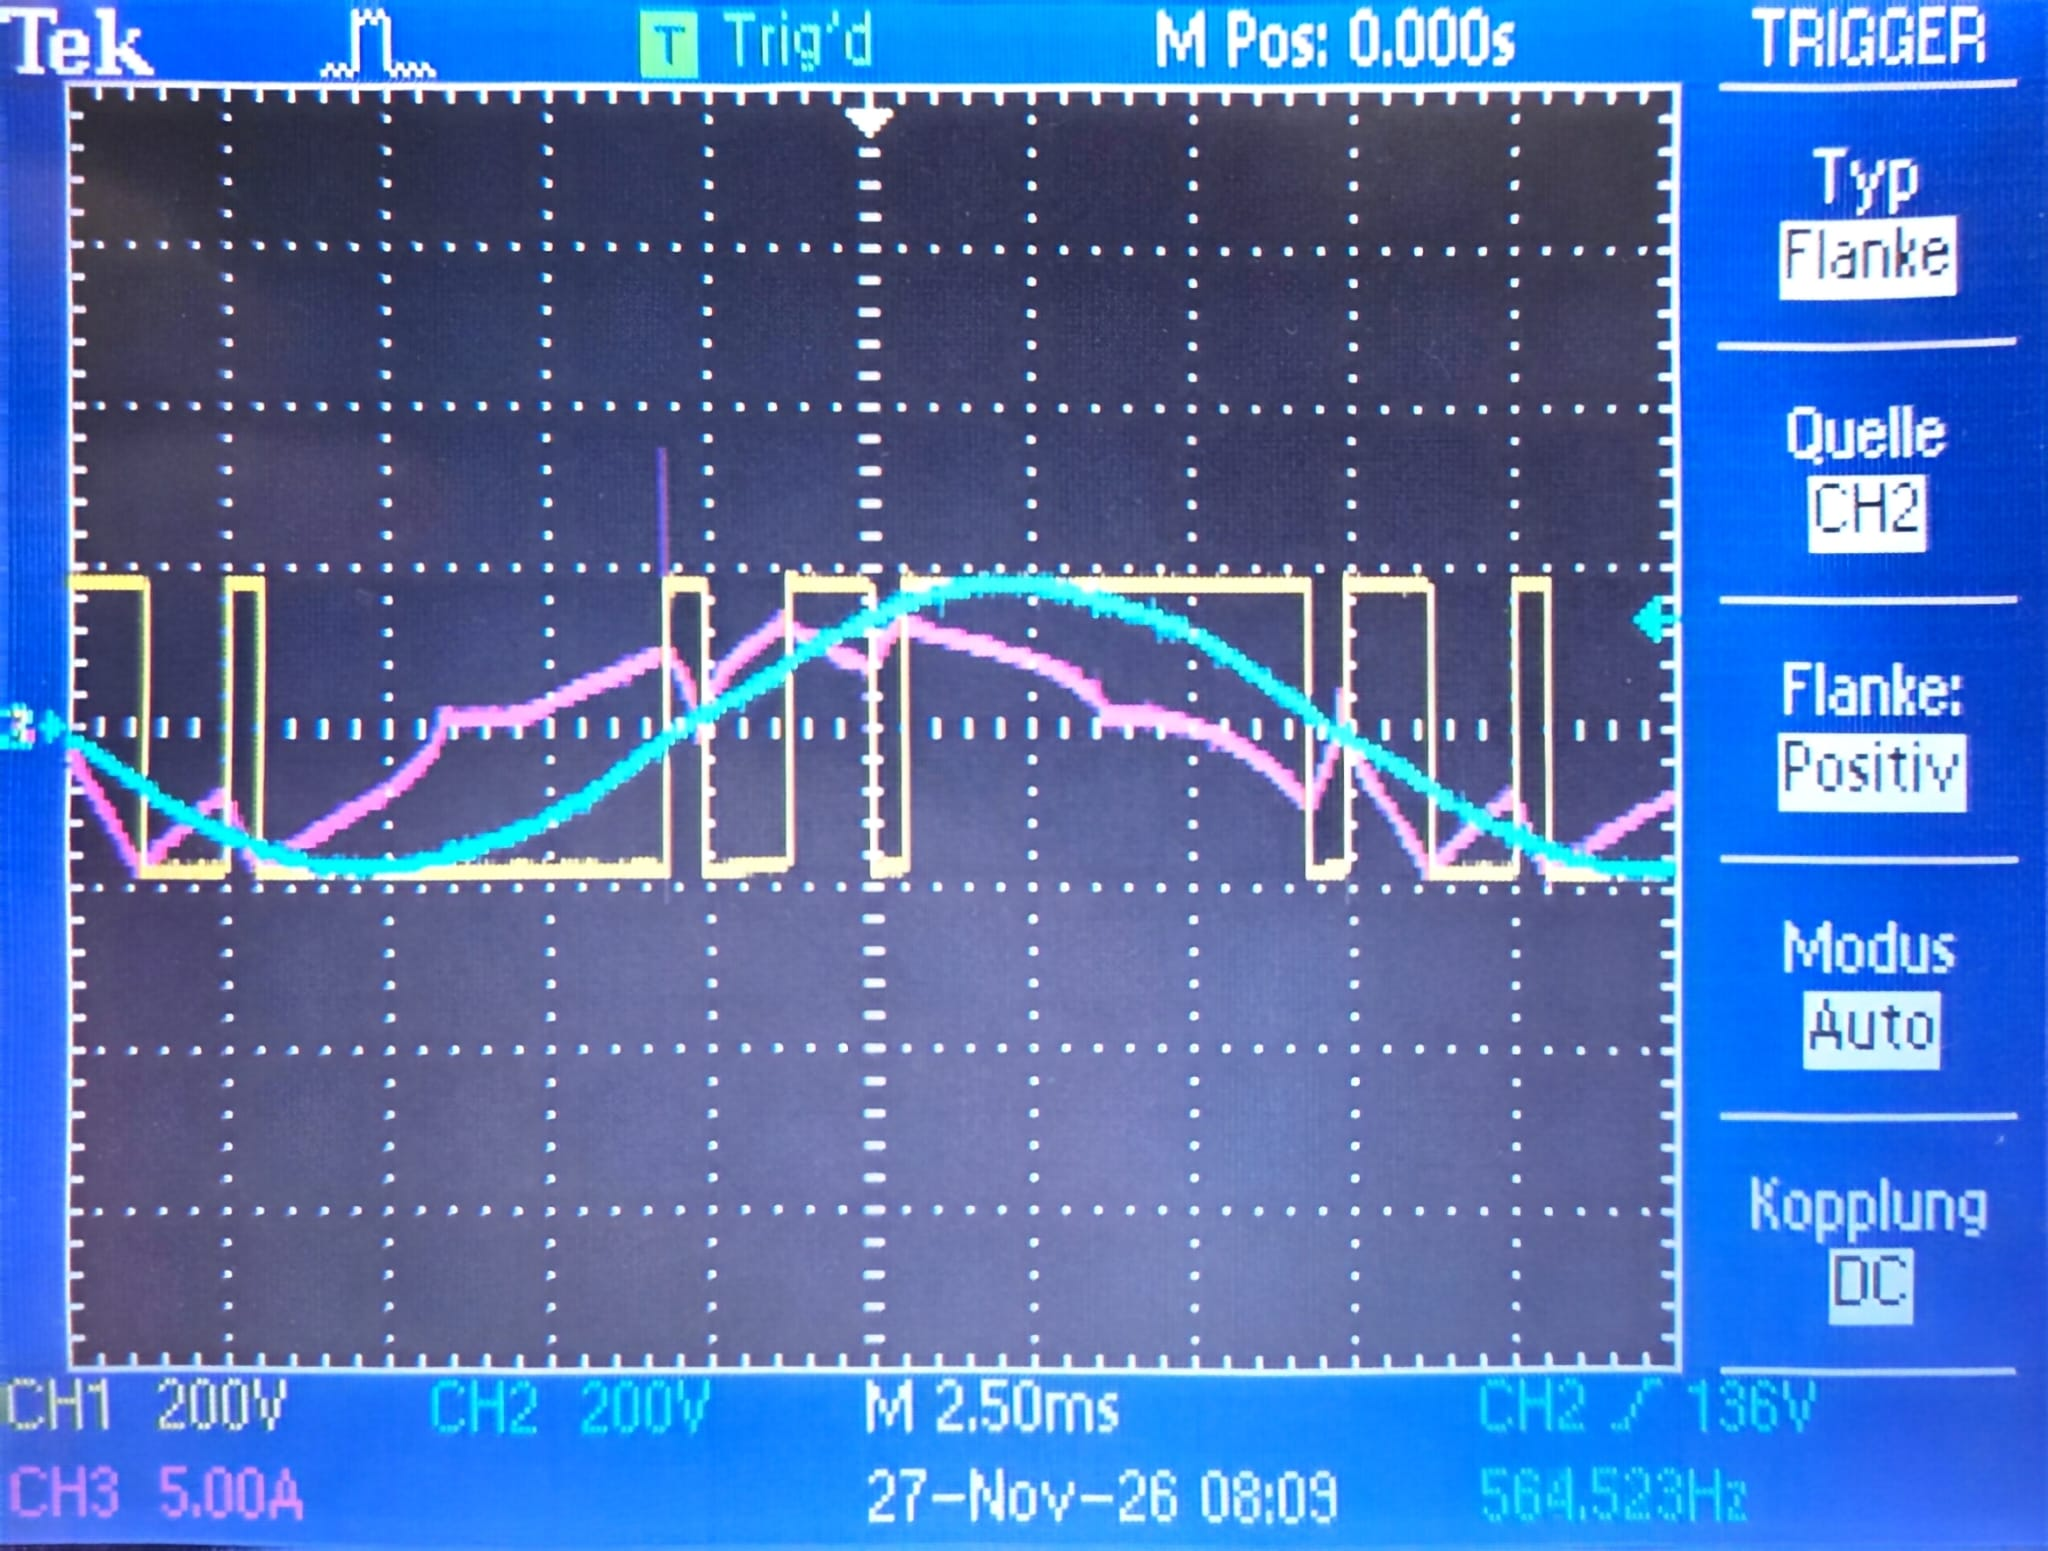
\includegraphics[width=\linewidth]{3_5_eliminiert.jpeg}
    \caption{«3.\ und 5.\ eliminiert», $\Udc=\SI{342}{\volt}$, $\Th=\SI{29.8}{\degree}$ (27.11.2026)}
    \label{fig:621_elim}
  \end{subfigure}\hfill
  \begin{subfigure}[t]{0.48\linewidth}
    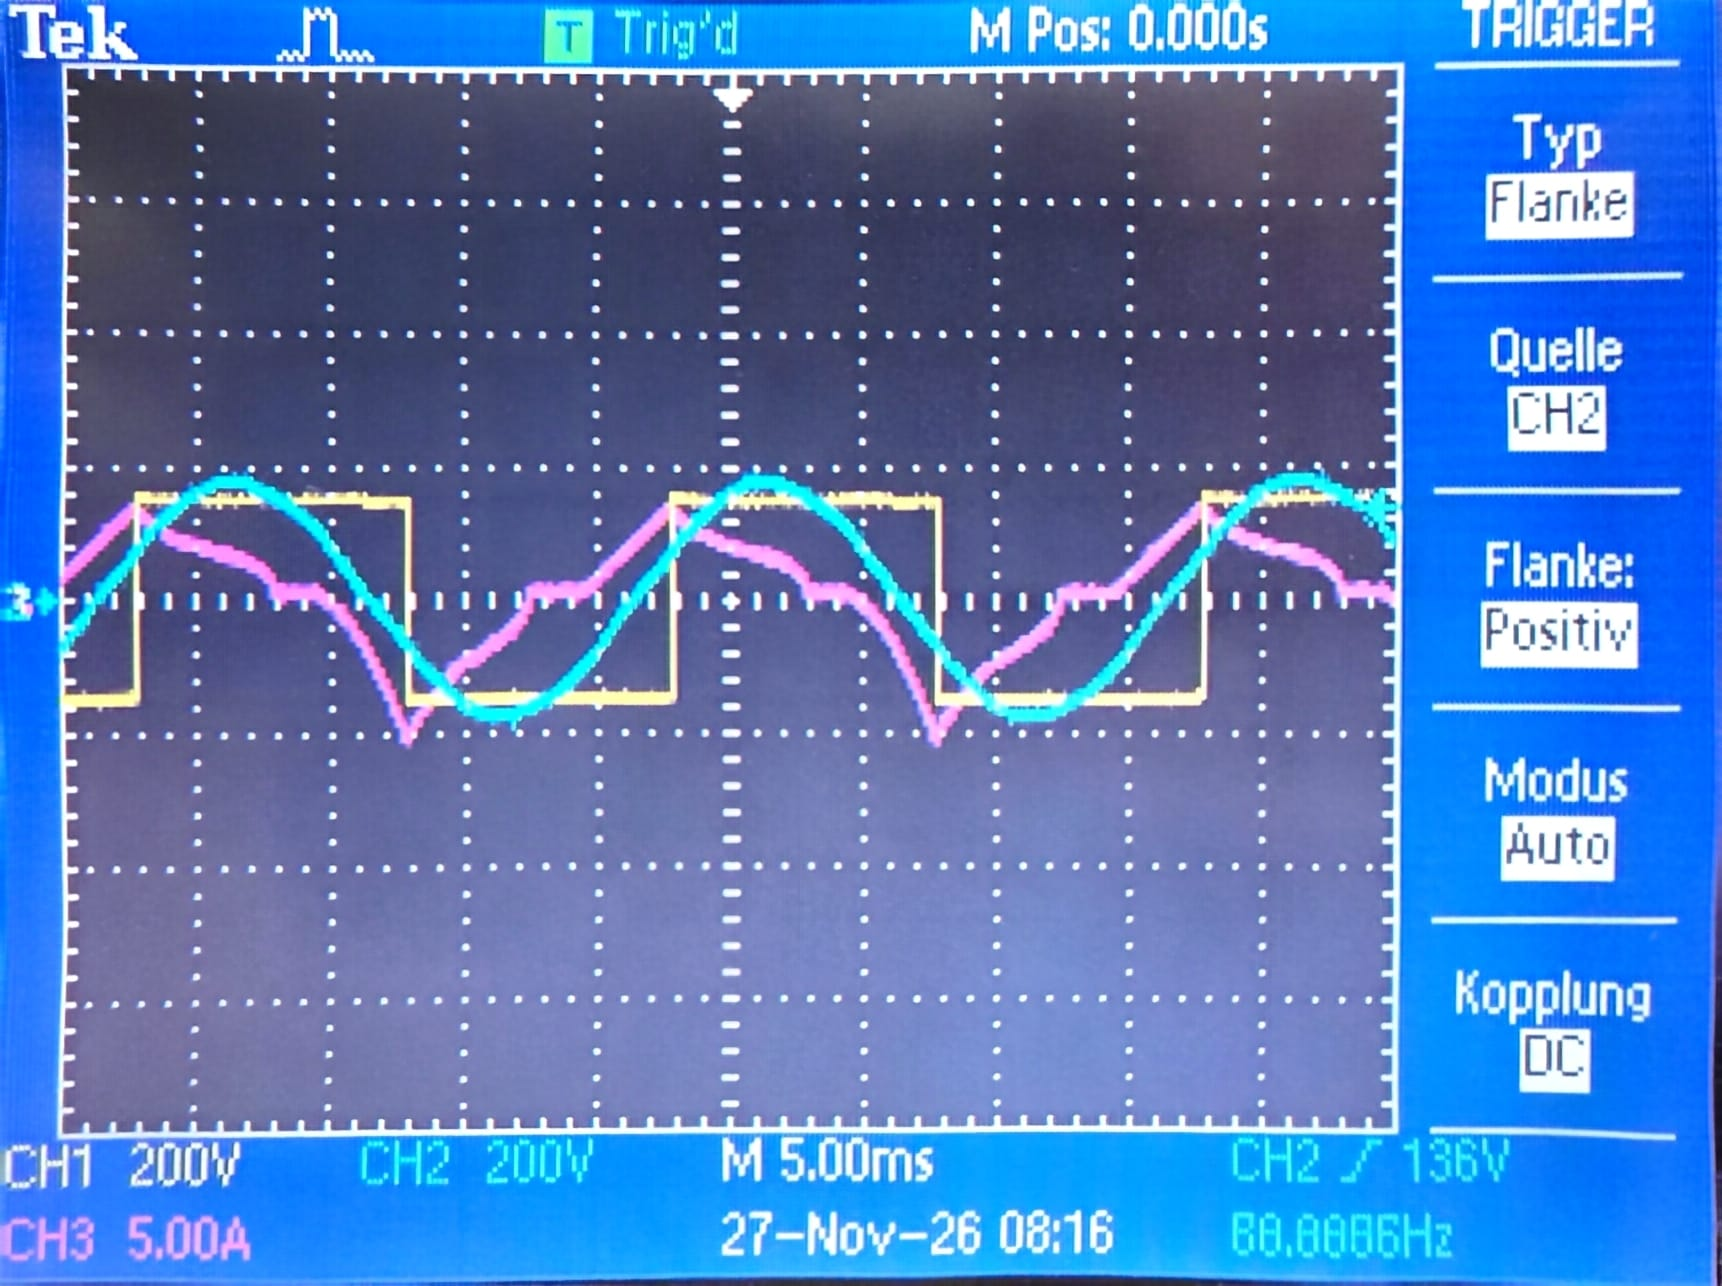
\includegraphics[width=\linewidth]{Grundferquenztaktung.jpeg}
    \caption{Grundfrequenztaktung (Referenz), $\Udc=\SI{284}{\volt}$, $\Th=\SI{28}{\degree}$ (27.11.2026, \SI{5}{\milli\second}/div)}
    \label{fig:621_rechteck}
  \end{subfigure}
  \caption{Oszillogramme am Lastpunkt $P\approx\SI{1.15}{\kilo\watt}$, $Q_1\approx0$. (a) und (b) vom 20.11.2026: Wechselrichterspannung (Cyan), Netzspannung (Gelb), Netzstrom (Magenta). (c) und (d) aus der Nachmessung vom 27.11.2026: Wechselrichterspannung (Gelb), Netzspannung (Cyan), Netzstrom (Magenta). Skalen: \SI{200}{\volt}/div, \SI{5}{\ampere}/div, \SI{2.5}{\milli\second}/div (Teilbild (d): \SI{5}{\milli\second}/div).}
  \label{fig:621}
\end{figure}

\paragraph{Beobachtungen.} Bei «3.\ und 5.\ eliminiert» ist $U_3=\SI{0.5}{\percent}$, die Elimination der 3.\ Oberschwingung ist damit bestätigt. Der gemessene Wert $U_5=\SI{30}{\percent}$ widerspricht der Erwartung (nahezu null); angesichts der stark schwankenden Anzeige (siehe unten) ist er vermutlich ein Ablesefehler. Dass $I_3=\SI{9}{\percent}$ trotz $U_3\approx0$ nicht verschwindet, könnte an einer Oberschwingung der Netzspannung liegen (Vermutung, $u_{\mathrm N}$ wurde nicht ausgewertet). Beim Trägerverfahren sind $U_3=\SI{20}{\percent}$ bzw.\ \SI{30}{\percent} unerwartet hoch, denn die Oberschwingungen sollten um die Schaltfrequenz liegen. Mögliche Ursachen sind Übermodulation (wenn die Grundschwingung am Rand des Aussteuerbereichs liegt), Ablesefehler oder ein anderer Prozentbezug (Vermutungen).

\paragraph{Messunsicherheit der Oberschwingungen.} Die Anzeige der Oberschwingungen am PM\,3000 schwankte bei den Pulsmustern stark; die abgelesenen Anteile streuten zwischen etwa \SI{2}{\percent} und \SI{50}{\percent}. Pro Grösse wurden deshalb mehrere Werte abgelesen und ungefähr gemittelt. Die Prozentwerte in Tabelle~\ref{tab:621_harm} sind daher nur grobe Richtwerte, und ein Vergleich der Muster auf wenige Prozentpunkte genau ist damit nicht möglich.

\paragraph{Stromformen.} Auf den Oszillogrammen ist der Unterschied der Muster gut zu sehen. Bei Grundfrequenztaktung (Abbildung~\ref{fig:621_rechteck}) ist der Strom stark verzerrt und hat bei jeder Schaltflanke eine Spitze. Beim Trägerverfahren «fein» besteht $\uWR$ aus einer sehr dichten Pulsfolge, und der Netzstrom verläuft nahezu glatt mit kleinem Schaltrippel. Bei «grob» gibt es deutlich weniger Pulse pro Netzperiode; der Strom ist sichtbar zackig und knickt bei jeder Schaltflanke. Beim Muster «3.\ und 5.\ eliminiert» (Abbildung~\ref{fig:621_elim}) ist $\uWR$ eine Rechteckspannung, in die an beiden Enden jeder Halbperiode zwei schmale Kerben geschnitten sind; die breite Mitte der Halbperiode bleibt erhalten. Der Strom ist dreieckförmig, mit einem Knick bei jeder Kerbe, und weniger spitz als bei Grundfrequenztaktung. Qualitativ ist der Strom bei «fein» damit am glattesten, was zur Theorie passt; die abgelesenen Prozentwerte zeigen das wegen ihrer Streuung nicht.

% ==========================================================================
\subsection{Aufgabe 6.2.2: Einstellen von \texorpdfstring{$P$ und $Q$}{P und Q} beim besten Muster}
\label{sec:messung622}

Die $P/Q$-Messungen für das beste Muster wurden aus Zeitgründen nicht durchgeführt.

\paragraph{Abschätzung von $\cos\varphi$ und $\lambda$.} Am Lastpunkt ist $Q_1\approx0$, also $\cos\varphi_1\approx1$. Der Leistungsfaktor $\lambda=P/S$ ist wegen der Oberschwingungsströme kleiner; bei sinusförmiger Netzspannung gilt $\lambda=\cos\varphi_1/\sqrt{1+\mathrm{THD}_I^2}$. Aus den abgelesenen $I_3$ und $I_5$ (Tabelle~\ref{tab:621_harm}) lässt sich $\mathrm{THD}_I$ nur nach unten abschätzen, weil die höheren Ordnungen fehlen; $\lambda$ ist damit eine obere Schranke (Tabelle~\ref{tab:622}). Wegen der Streuung der abgelesenen Werte sind das nur Grössenordnungen.

\begin{table}[htbp]
  \centering
  \caption{Abschätzung von $\mathrm{THD}_I$ und $\lambda$ aus $I_3$ und $I_5$ (berechnet, nicht gemessen; $\cos\varphi_1\approx1$).}
  \label{tab:622}
  \begin{tabular}{@{}lrr@{}}
    \toprule
    Pulsmuster & $\mathrm{THD}_I\gtrsim$ & $\lambda\lesssim$ \\
    \midrule
    3.\ und 5.\ eliminiert & \SI{11}{\percent} & 0.99 \\
    Trägerverfahren grob & \SI{24}{\percent} & 0.97 \\
    Trägerverfahren fein & \SI{36}{\percent} & 0.94 \\
    \bottomrule
  \end{tabular}
\end{table}

% ==========================================================================
\subsection{Aufgabe 6.3: Spannungsbelastung der Halbleiter}
\label{sec:messung63}

Erwartet wird für einen Halbleiter des Wechselrichters Folgendes (Skizze in Abbildung~\ref{fig:halbleiter_skizze}): Die Spannung über dem Schalter ist null, solange er leitet, und gleich der vollen Zwischenkreisspannung $\Udc$, solange er sperrt. Beim Schalten können Überschwinger auftreten. Der Strom entspricht im Leitintervall dem Netzstrom $\iN$; je nach Stromrichtung führt ihn der IGBT oder die antiparallele Diode.

\begin{figure}[htbp]
  \centering
  \begin{tikzpicture}
    \begin{axis}[rep,height=3.6cm,xlabel={},ylabel={$u_{\mathrm T}$},
        xmin=0,xmax=360,xtick={0,90,...,360},ymin=-0.2,ymax=1.3,ytick={0,1},yticklabels={0,$\Udc$}]
      \addplot[thick,domain=0:360,samples=721]{ifthenelse(x<180,0,1)};
    \end{axis}
  \end{tikzpicture}

  \begin{tikzpicture}
    \begin{axis}[rep,height=3.6cm,xlabel={$\omega t$ in \si{\degree}},ylabel={$i_{\mathrm T}$ in A},
        xmin=0,xmax=360,xtick={0,90,...,360},ymin=-5,ymax=5]
      \addplot[thick,domain=0:360,samples=721]{ifthenelse(x<180,(255.46*(x*pi/180-pi/2)+325.27*cos(x))/21.99,0)};
    \end{axis}
  \end{tikzpicture}
  \caption{Skizze (Erwartung) von Spannung $u_{\mathrm T}$ und Strom $i_{\mathrm T}$ des oberen Schalters für den Fall aus Abschnitt~\ref{sec:vorbereitung}: Der Strom fliesst im Leitintervall; seine positiven Anteile laufen über den IGBT, die negativen über die Diode (je nach Stromrichtung).}
  \label{fig:halbleiter_skizze}
\end{figure}

\begin{figure}[htbp]
  \centering
  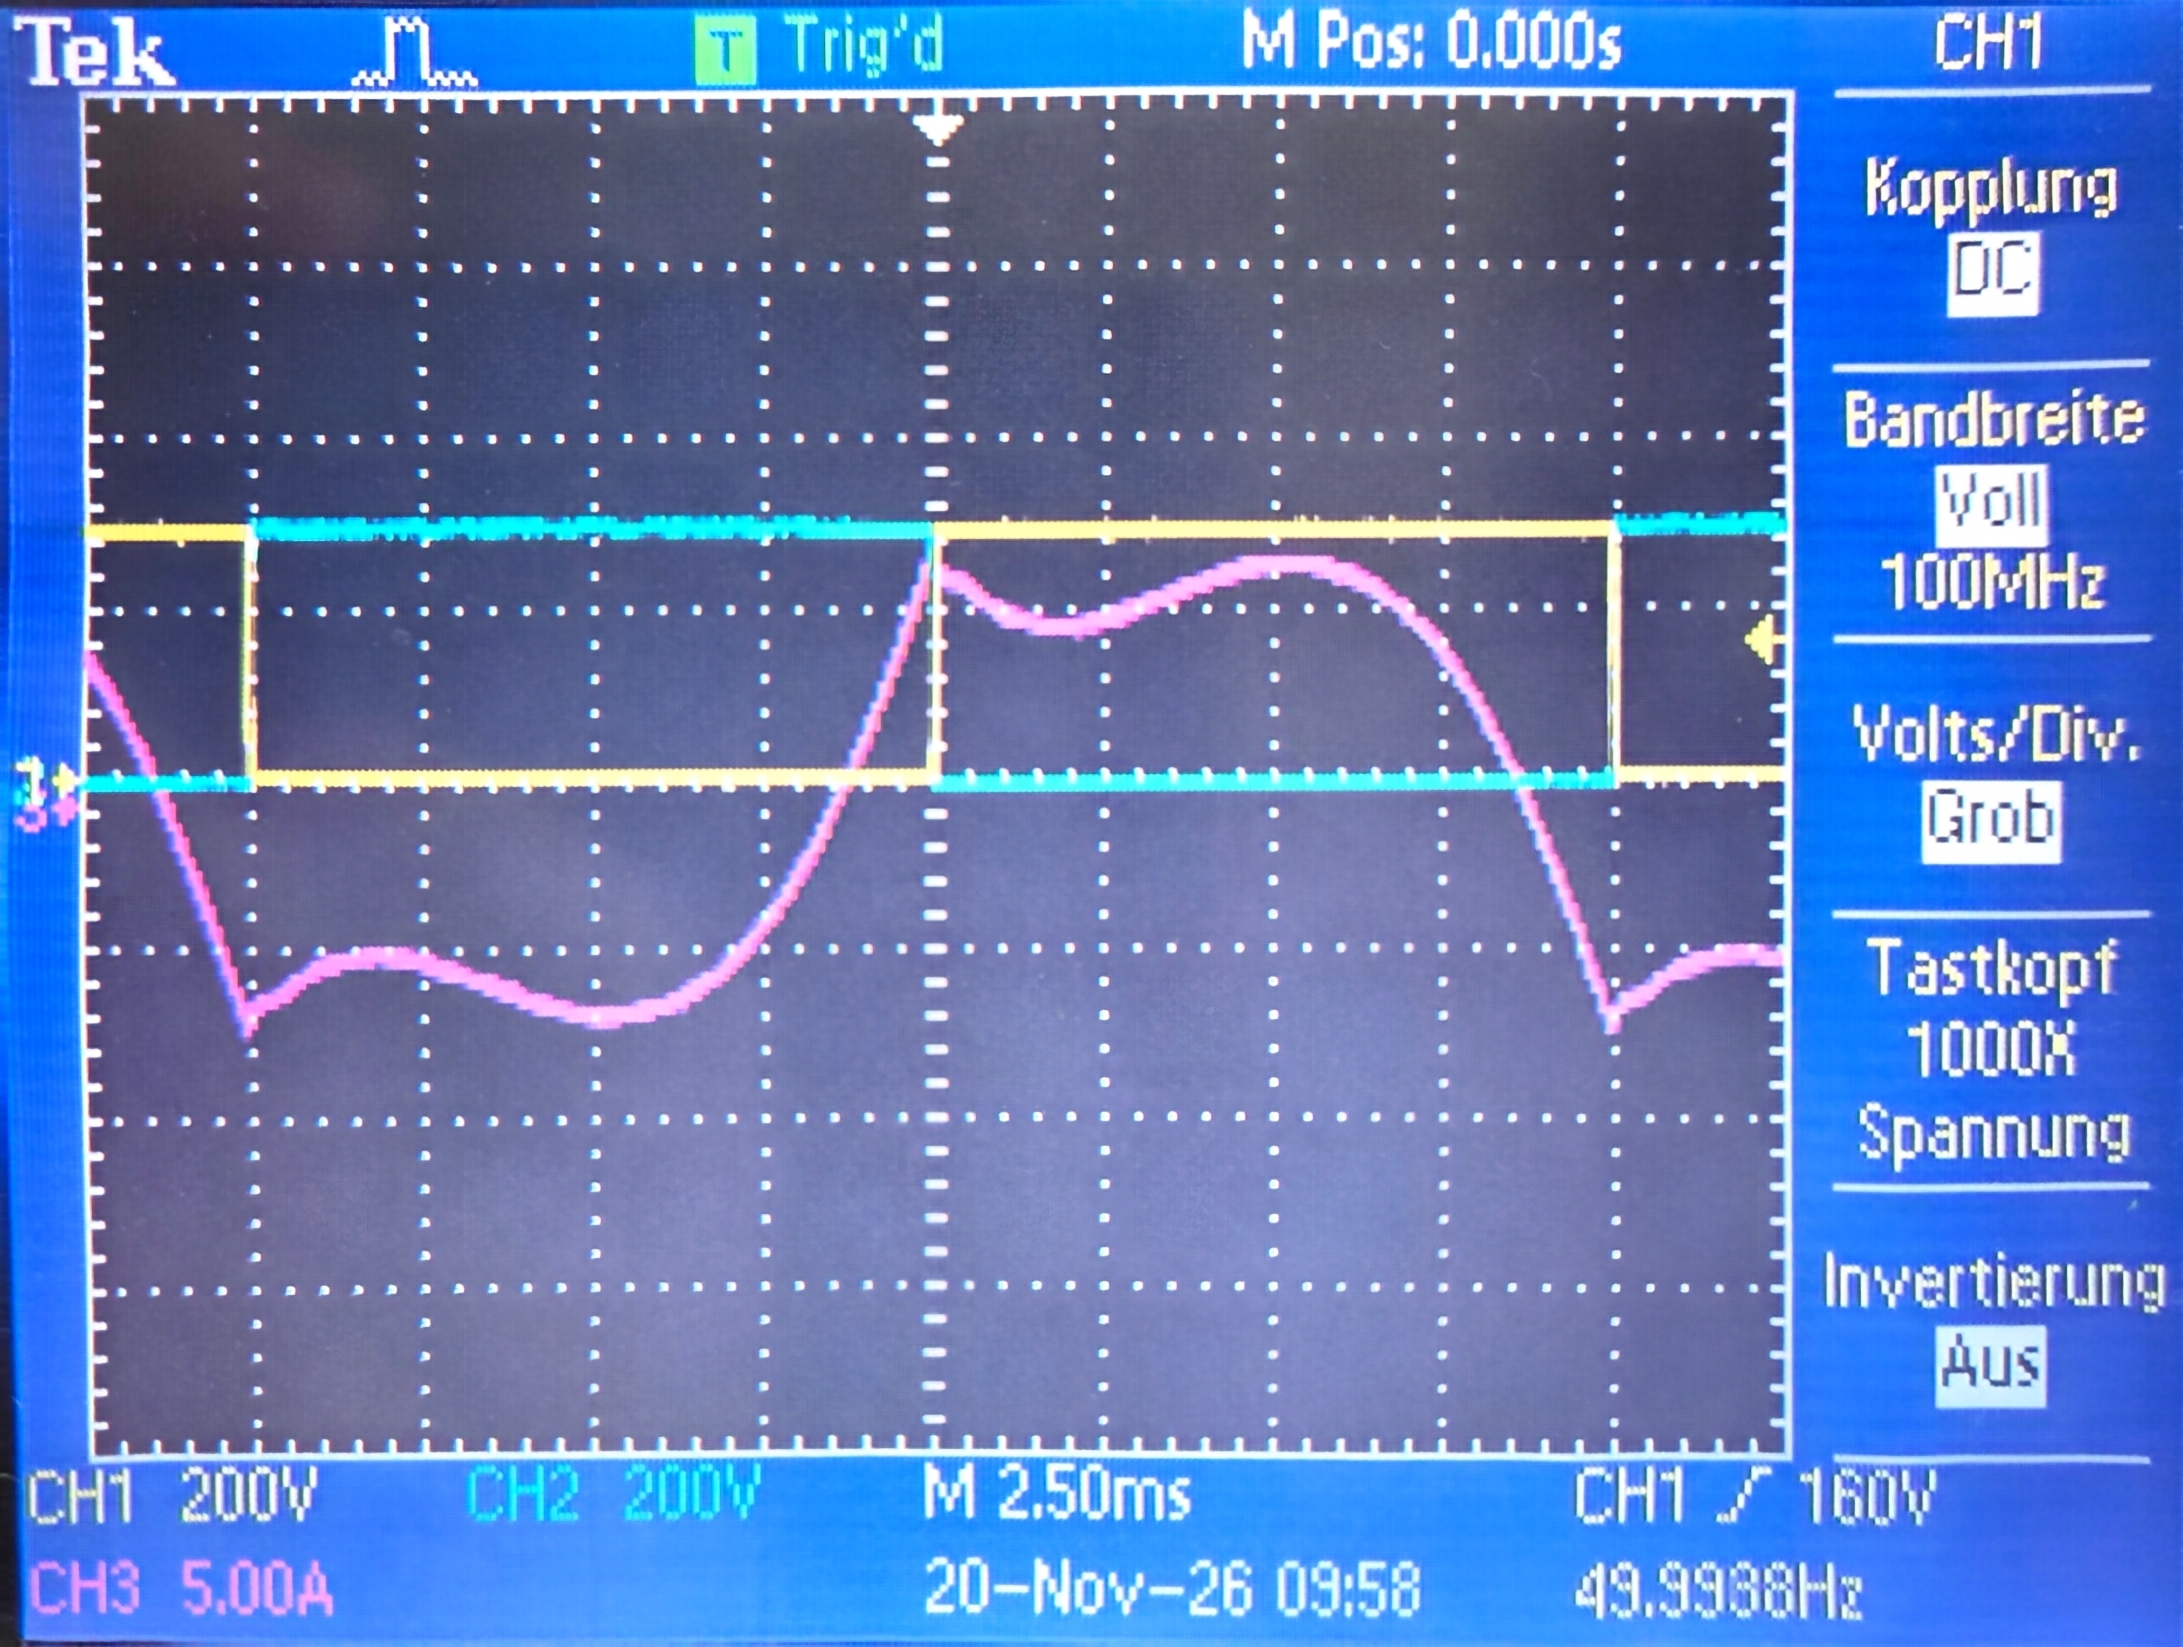
\includegraphics[width=0.62\linewidth]{Scan_20261120_102240.jpg}
  \caption{Aufgabe 6.3, Oszillogramm (20.11.2026, 09:58). Skalen: \SI{200}{\volt}/div (CH1, CH2), \SI{5}{\ampere}/div (CH3), \SI{2.5}{\milli\second}/div.}
  \label{fig:halbleiter_mess}
\end{figure}

Gemessen wurde bei Grundfrequenztaktung. Das Oszillogramm zeigt zwei zueinander komplementäre Rechteckspannungen (Gelb, Cyan) mit einem Hub von rund \SI{290}{\volt}, was der Zwischenkreisspannung entspricht. Es sind die Spannungen über zwei Halbleitern, und zwar Cyan über dem Schalter, der die positive Halbwelle von $\uWR$ schaltet, und Gelb über dem Schalter der negativen Halbwelle. Magenta ist der Netzstrom $\iN$. Die Flanken sind sauber, bei \SI{200}{\volt}/div sind keine Überschwinger zu erkennen. Der Netzstrom ändert bei jeder Schaltflanke seine Steigung, wie es $L\,\mathrm{d}i/\mathrm{d}t=\uWR-\uN$ verlangt; er fliesst durch den Halbleiter, solange dieser leitet.

% ==========================================================================
\subsection{Aufgabe 6.4: Drehzahl der Asynchronmaschine}
\label{sec:messung64}

Die Drehzahl wurde mit dem optischen Drehzahlmesser gemessen. Tabelle~\ref{tab:drehzahl} stellt die gemessenen Werte den Angaben auf dem Typenschild gegenüber. Im Leerlauf wurden \SI{1500}{\per\minute} gemessen; das entspricht der Synchrondrehzahl und dem Wert auf dem Typenschild.

\begin{table}[htbp]
  \centering
  \caption{Drehzahl der ASM: gemessene Werte und Angaben auf dem Typenschild.}
  \label{tab:drehzahl}
  \begin{tabular}{@{}llr@{}}
    \toprule
    Zustand & Quelle & $n$ in \si{\per\minute} \\
    \midrule
    Leerlauf & gemessen & 1500 \\
    Nennlast & Typenschild & 1430 \\
    Generatorbetrieb, $P\approx\SI{1.1}{\kilo\watt}$ & gemessen & 1505 \\
    Motorbetrieb, $P\approx\SI{-1.1}{\kilo\watt}$ ($\Th=\SI{-15}{\degree}$, $\Udc=\SI{288}{\volt}$) & gemessen & 1488.8 \\
    \bottomrule
  \end{tabular}
\end{table}

Der Betriebszustand der ASM folgt aus der Leistungsrichtung (Abschnitt~\ref{sec:vorzeichen}). Bei $P>0$ arbeitet der Wechselrichter als Gleichrichter und treibt die GM als Motor an; die ASM wird dann übersynchron angetrieben und arbeitet als Generator, hier bei \SI{1505}{\per\minute}. Bei $P<0$ speist der Wechselrichter in das Netz~2 zurück, die GM ist Generator und die ASM Motor; sie läuft untersynchron, hier bei \SI{1488.8}{\per\minute}. Die lastpunktbezogenen Messungen der übrigen Aufgaben fanden im Generatorbetrieb statt; der Motorbetrieb wurde nur für diese Drehzahlmessung durch Ändern des Winkels eingestellt.

Gemessen liegt die Drehzahl damit zwischen etwa \SI{1489}{\per\minute} und \SI{1505}{\per\minute}, also nur rund $\pm\SI{0.5}{\percent}$ um die Synchrondrehzahl von \SI{1500}{\per\minute}; die ASM hält die Drehzahl wie vorausgesetzt praktisch konstant. Daraus ergibt sich im Motorbetrieb ein Schlupf von $s=(1500-1488.8)/1500\approx\SI{0.75}{\percent}$ und im Generatorbetrieb von $s\approx\SI{-0.33}{\percent}$ (berechnet). Der Typenschildwert von \SI{1430}{\per\minute} bei Nennlast entspricht einem Schlupf von rund \SI{4.7}{\percent}; er wurde nicht gemessen, da die Nennlast nicht gefahren wurde. Die Synchrondrehzahl von \SI{1500}{\per\minute} bei \SI{50}{\hertz} entspricht der Polpaarzahl $p=2$; diese wurde aus der Drehzahl abgeleitet und nicht auf dem Typenschild geprüft.
